\chapter {Technische Machbarkeit}
Die Technische Machbarkeit in dem Sinne ist das Gegenstück der Wirtschaftlichen Machbarkeit.
Hier werden die wissenschaftlichen Informationen, die zur Umsetzung des Projektes beitragen,
gesammelt. 

\section {Varianten}
Das Projekt BestShift umfasst eine Reihe an Anforderungen, die innerhalb des Teams verteilt sind.

\section{Programmiersprache}
Bei den Programmiersprachen bestand die Auswahl zwischen Framework Python, 
native Java und Hybrid mit Java und HTML.
Dabei fiel für uns vor allem aufgrund von der Verbindung mit einer Webapplikation die Wahl auf eine hybride Applikation. 

\newpage
\subsection{Vergleich Java und Python}
\subsubsection{Java}
\begin{itemize}
\item Charakteristik: Mehrfachverwendung/Mehrfachvererbung eingeschränkt, stark typisiert
\item Syntax: Vor der Kompilierung sehr streng, komplizierte Polymorphie
\item Dokumentation: Ausführliche Dokumentation der Methoden in Form von Java API
\item Community: Java ist sehr weit verbreitet, rund 3 Milliarden Geräte können Java auführen.
\item Usage: plattformunabhängige Programme, FAT-Client-Anwendungen
\item Können im Team: 5/5*, jahrelange Erfahrung innerhalb des Teams
\end{itemize}

\subsubsection{Python}
\begin{itemize}
\item Charakteristik: Erstellung von Variablen nicht Datentyp abhängig, dynamisch/schwach typisiert.
\item Syntax: erhöhte Lesbarkeit im Vergleich zu allen anderen, aber ungewohnter zu schreiben als Java
\item Dokumentation: innerhalb der Python API vorhanden.
\item Community: Die Community von Python ist ständig am wachsen, ca. 5 Millionen Geräte verwenden Python.
\item Usage: Back-End, äußerst schnelle Entwicklung(Rapid Application Development)
\item Können im Team: 3/5*, Team konnte erst geringe Erfahrung mit Python sammeln
\end{itemize}

Aus den Oben genannten Punkten filtern wir heraus, dass Java die bessere Lösung für die Android App wäre. 
Die komplette Beherrschung von Python würde einige Wochen dauern. 
Da diese Zeit im Rahmen des Diplomprojektes nicht vorhanden ist, wäre die App-Entwicklung in Python nicht zielführend. 
Außerdem benutzen Android-Smartphones die Dalvik-VM, welche Java Class Files exekutiert, 
wodurch Java nativ auf Android realisiert wird im Gegensatz zu Python. 
Dementsprechend wird hier massiv an Umkompilierungszeit gespart, welche für die Echtzeit-Darstellung des Verbrauchs, 
Kamm'schen Kreises und Schaltvorschlags essentiell ist.
\subsection{Java-Frameworks(APP)}
\newline
\begin{table}[!htb]
\centering
\caption{Vergleich der Charting-Frameworks}
\label{comparisonCharting}
\resizebox{\columnwidth}{!}{%
\begin{tabular}{l|c|c|c|l|}
\cline{2-5}
 & \begin{tabular}[c]{@{}c@{}}MPAndorid\\ Chart\end{tabular} & \begin{tabular}[c]{@{}c@{}}AChart\\ Engine\end{tabular} & HelloChart & Erklärung \\ \hline
\multicolumn{1}{|l|}{Performance} & Gut & Gut & Gut &  \\ \hline
\multicolumn{1}{|l|}{\begin{tabular}[c]{@{}l@{}}Supported \\ Languages\end{tabular}} & \begin{tabular}[c]{@{}c@{}}iOS 7,8;\\ Java\end{tabular} & Java & Java & \begin{tabular}[c]{@{}l@{}}MPAC kann auch\\ weiterverwendet werden\\ für eine iOS App\end{tabular} \\ \hline
\multicolumn{1}{|l|}{Documentation} & 85\% & 70\% & 50\% & \begin{tabular}[c]{@{}l@{}}MPAC hat eine sehr gute\\ in Kapiteln aufgelistete\\ Dokumentation, Tutorials\end{tabular} \\ \hline
\multicolumn{1}{|l|}{Recent activity} & 19.10.2015 & 26.07.2013 & 5.10.2015 & \begin{tabular}[c]{@{}l@{}}MPAC ist sehr aktuell\\ und bringt immer wieder \\ neue Bugfixes raus.\\ HelloChart ebenso.\end{tabular} \\ \hline
\multicolumn{1}{|l|}{Community} & 80\% & 60\% & 20\% & \begin{tabular}[c]{@{}l@{}}Bei MPAC und \\ AChartEngine wird eine\\ Antwort innerhalb von 7 \\ Tagen geliefert.\\ Eine Community bei Hello\\ Chart ist kaum vorhanden.\end{tabular} \\ \hline
\multicolumn{1}{|l|}{Usage examples} & 85\% & 70\% & 15\% & \begin{tabular}[c]{@{}l@{}}MPAC hat für jeden Chart\\ ein eigenes Beispiel oder \\ auch Tutorials auf YouTube.\\ AChartEngine weniger \\ verwendbare Codebeispiele.\end{tabular} \\ \hline
\end{tabular}
}
\end{table}

Im Großen und Ganzen ist MPAndroidChart das Beste was man wählen kann, da es eins der besten Dokumentationen hat, weiterhin hat es auch eine sehr gute Community, sehr viel gut gecodete und Dokumentierte Beispiele und ist auch für Erweiterung gut , da die App auch auf einem IPhone programmiert werden kann. 
AChartEngine hat eine gute Dokumentation doch eine eher schwächere Community und ist leider nicht sehr aktuell. 
HelloChart hat eins der schlechtesten Dokumentationen, gar keine Community und sehr wenig gecodete Beispiele, sie sind aber sehr Aktuell wenn es um die Versionen geht .
 
\newpage

\subsection{Python-Frameworks(Web-Applikation)}
\newline
\begin{table}[!htb]
\centering
\caption{Vergleich der Charting-Frameworks}
\label{comparisonCharting}
\resizebox{\columnwidth}{!}{%
\begin{tabular}{l|c|c|c|l|}
\cline{2-5}
 & \begin{tabular}[c]{@{}c@{}}Plotly \end{tabular} & \begin{tabular}[c]{@{}c@{}}Chart.js\end{tabular} & HelloChart & Erklärung \\ \hline
\multicolumn{1}{|l|}{Performance} & Gut & Gut & Gut &  \\ \hline
\multicolumn{1}{|l|}{\begin{tabular}[c]{@{}l@{}}Supported \\ Languages\end{tabular}} & \begin{tabular}[c]{@{}c@{}}
Python \end{tabular} & Python & Python & \begin{tabular}[c]{@{}l@{}} \end{tabular} \\ \hline
\multicolumn{1}{|l|}{Documentation} & 90\% & 60\% & 70\% & \begin{tabular}[c]{@{}l@{}}Plotly hat die Beste Docu\\ von allen \\Von allen Chartarten bis Tutorials\\und Code\\ Chart.js hat eine\\ eher Mittelmäßige Docu \end{tabular} \\ \hline
\multicolumn{1}{|l|}{Recent activity} & Release 2.5 & Release 2.0 beta & Release 2.0 & \begin{tabular}[c]{@{}l@{}}Plotly hat \\ sehr viele \\ Releases rausgebracht.\end{tabular} \\ \hline
\multicolumn{1}{|l|}{Community} & 70\% & 50\% & 30\% & \begin{tabular}[c]{@{}l@{}}Plotly hat \\ eine sehr gute Community\\ in der erstellte Grafen\\hochgestellt werden\\ .\end{tabular} \\ \hline
\multicolumn{1}{|l|}{Usage examples} & 90\% & 60\% & 15\% & \begin{tabular}[c]{@{}l@{}}Da Plotly eins der besten \\ Dokumentationen hat\\ ist es nicht sehr \\leicht zu erlernen.\end{tabular} \\ \hline
\end{tabular}
}
\end{table}

Plotly hat eins der Besten Dokumentationen die wir bis jetzt gesehen haben. Sie haben eine sehr große Auswahl an Charts, welche mit Code zur verfügung stehen. 
Weiters haben sie tutorials, Dokumentationen unterteilt in Kapitel. Weiterhin ist das Framework sehr weit entwickelt worden.                  
Eins der Nachteile wäre, dass wir keine SVG Images exportieren können. Für einen Betrag von 20euro Monatlich ist auch das möglich. 
Ich bin zum Entschluss gekommen, dass Plotly das Beste Framework für unsere Webapplikation sein könnte, 
da sehr viel Dokumentiert, Gecodet wurde, außerdem ist es das am leichtesten erlernbare Tool.


\newpage

\subsection{Hybrid-Frameworks}
Es fällt die Auswahl auf eines der folgenden Frameworks:
\begin{itemize}
\item \hyperref[Codename One]{https://www.codenameone.com/pricing.html} Java
\item \hyperref[Firebase]{https://www.firebase.com/pricing.html} Android/iOS/JavaScript SDK
\item \hyperref[appmethod]{http://www.appmethod.com/de/pricing} C++
\item \hyperref[ionic]{http://ionicframework.com/} HTML, CSS, JS; Built with Sass, optimized with AngularJS
\end{itemize}

\textit{Dokumentation}
Alle sind gut dokumentiert, Codename One und Firebase bieten sogar eine eingeschränkte kostenlose Option.
ionic ist von sogar OpenSource und hat eine tolle einsteigerfreundliche Dokumentation

\textit{Usage/Charakteristika}
\begin{itemize}
\item Codename One bietet eine Java SDK um eine App welche auf iOS, Windows oder Android lauffähig ist
\item Firebase bietet eine Android, iOS und JavaScript SDK um eine vielseitig kompatible mobile oder web Applikation zu entwickeln. 
\item Mittels appmethod kann man mit einer C++ Codebasis eine Android, iOS, MacOSX und sogar eine Windows Applikation entwickeln.
\item Bei ionic wird die App von einer mobil-freundlichen HTML, CSS und JS Library entwickelt, während sie dann mit Sass auf das jeweilige App Format konvertiert wird und mit Angular JS optimiert wird. 
\end{itemize}

\textit{Community}
\begin{itemize}
\item Codename One bietet einen Blog, eine in die Webseite eingebundene Google Discussion und einen Stackoverflow codenameone-Tag.
\item Firebase hat einen Blog und über 25000 Facebook likes, aber sonst leider nur ein GitHub um Issues zu publizieren und eigene Support Emails, also ist hier alles sehr zentralisiert gesteuert. 
\item appmethod hat eine Github page, welche aber ebenfalls eher durch den Support mit Issues gefüllt wird und verlinkt für die Community auf die Homepage der Mutterfirma \"Embarcadero\", welche auch ein Forum anbieten
\item ionic hat eine großes community-driven Forum, welches bei vielen Beiträgen mehrere hundert Antworten als Wissenserweiterung anbietet.
\end{itemize}

\newpage
\textit{Performance}
\begin{itemize}
\item Codename One verwendet SaaS für die Kompilierung der App und verwendet eine VM die Java zu C für iOS macht. Die Performance ist hoch da es die nativen gaming Plattformen des jeweiligen OS verwendet. 
\item Firebase verwendet die Forge UI und ist dadurch auf große Datensätze sogar ausgelegt, nur muss man achten diese zu denormieren.
\item Da appmethod C++ als Programmiersprache verwendet, welche direkt auf der CPU laufen kann, appmethod performant.
\item In einem Post von Sep.2014 wird ionic als weniger performant gesehen. Document Object Model (DOM) sollten möglichst selten angezeigt werden um gute Performance und Seite zu Seite Wechsel sollten auch unterlassen werden. Allerdings scheint das ionic Team sehr Performance fokussiert zu sein.
\end{itemize}

\textit{Last Update}
\begin{itemize}
\item Codename One: neuester Blogbeitrag: 14.10.2015
\item Firebase: Github letzter Commit: vor 14 Stunden
\item appmethod: Github letzter Commit: 21.09.2015
\item ionic: Github letzter Commit: 14.10.2015
\end{itemize}

\textbf{Frameworks Conclusio}
Es war grundsätzlich für uns bereits von Beginn an klar dass wir ein Framework verwenden würden, allerdings tendieren wir mittlerweile in die Richtung eines hybriden Frameworks. Codename One und appmethod fallen aufgrund ihrer mangelnden kostenfreien Option definitiv weg. Ionic und Firebase scheinen schon weit interessanter.
Da muss man sich allerdings eine Grundsatzfrage stellen - möchten wir eine HTML hybride App bauen oder nur eine cross-platform App? Denn für eine HTML hybride App müssten wir Ionic verwenden, auch wenn einige von uns dafür definitiv AngularJS und JS im allgemeinen wiederholen müssten.

\newpage
\section{Datenmanagement \& Datenanalyse}

In dem folgenden Kapitel werden einige Technologien, Libaries & Packages, sowie generelle Software gegenübergestellt. Diese werden dann subjektiv bewertet, und die am besten geeignetsten werden für das Projekt verwendet.

\subsection{Datenmanagement}

\subsubsection{Vergleich NoSQL und relational}
\subsubsubsection{SQL Datenbanken}
\begin{itemize}
\item Typen: Nur eine Art mit kleinen Unterschieden
\item Data Storage Model: Individuele Einträge werden als Reihen (Rows) in Tabellen gespeichert, wobei jede Zelle spezifische Daten über diesen Eintrag beinhaltet. 
\item Schemas: Strukur und daten type sind im vorhinein festgelegt. Um diese Datenbank Struktur zu ändern muss diese zunächst offline gesetzt werden.
\item Skalierbarkeit: Ein einzelner Server muss hierfür mehr Rechenleistung erhalten um größeren Anspruchen nachzukommen. Es ist prinzipiell möglich SQL Datenbanken auf ein verteiltes System zu erstellen, hierfür werden aber sehr gute Kenntnise benötigt.
\item Data Manipulation: Mittels SELECT, INSERT oder UPDATE
\item Konsistenz: Gute konsistenz kann prinzipiell in allen gänglichen DBMS konfiguriert werden.
\end{itemize}

\subsubsubsection{NoSQL Datenbanken}


\begin{itemize}
\item Typen: Viele verschiedene, bspw. key-value, document-based, oder graph datenbank.
\item Data Storage Model: Hängt vom Typ der Datenbank ab.
\item Schemas: Typischerweise dynamich. Einträge können \'on-the-fly\' hinzugefügt werden.
\item Skalierbarkeit: Bei Bedarf kann ein Administrator einfach mehrere Cloud Instanzen hinzufügen. Die Datenbank an sich verteilt die Information auf die notwendige Server Anzahl
\item Data Manipulation: Durch Objektorientierte APIs
\item Konsistenz: Abhängig vom Product
\end{itemize}

\begin{table}[!htb]
\centering
\caption{Vergleich von NoSQL-Datenbanken}
\label{Vergleich von NoSQL-Datenbanken}
\resizebox{\columnwidth}{!}{%
\begin{tabular}{l|l|l|l|l|l|}
\cline{2-6}
 & \textbf{Cassandra} & \textbf{Couchbase} & \textbf{HBase} & \textbf{MongoDB} & \textbf{Riak} \\ \hline
\multicolumn{1}{|l|}{Performance} & gut & sehr gut & befridigend & sehr gut & befriedigend \\ \hline
\multicolumn{1}{|l|}{Supported languages} & \begin{tabular}[c]{@{}l@{}}Java\\ Python\\ PHP\\ JavaScript\\ etc.\end{tabular} & \begin{tabular}[c]{@{}l@{}}Java\\ JavaScript\\ PHP\\ Python\\ etc.\end{tabular} & \begin{tabular}[c]{@{}l@{}}Java\\ PHP\\ Python\\ etc.\end{tabular} & \begin{tabular}[c]{@{}l@{}}Java\\ JavaScript\\ PHP\\ Python\\ PowerShell\\ etc.\end{tabular} & \begin{tabular}[c]{@{}l@{}}Java\\ JavaScript\\ PHP\\ Python\\ etc.\end{tabular} \\ \hline
\multicolumn{1}{|l|}{Documentation} & 80\% & 90\% & 80\% & 90\% & 70\% \\ \hline
\multicolumn{1}{|l|}{Current release} & \begin{tabular}[c]{@{}l@{}}2.2.2\\ October 2015\end{tabular} & \begin{tabular}[c]{@{}l@{}}4.0\\ October 2015\end{tabular} & \begin{tabular}[c]{@{}l@{}}1.1.0.1\\ May 2015\end{tabular} & \begin{tabular}[c]{@{}l@{}}3.0.6\\ August 2015\end{tabular} & \begin{tabular}[c]{@{}l@{}}2.1.0\\ April 2015\end{tabular} \\ \hline
\multicolumn{1}{|l|}{Community} & 80\% & 85\% & 90\% & 90\% & 80\% \\ \hline
\multicolumn{1}{|l|}{Usage examples} & \begin{tabular}[c]{@{}l@{}}Cisco\\ eBay\\ PayPal\\ Verizon\\ Walmart\end{tabular} & \begin{tabular}[c]{@{}l@{}}Adobe\\ Facebook\\ Twitter\\ Yahoo\end{tabular} & \begin{tabular}[c]{@{}l@{}}Bosch\\ Forbes\\ Chicago Gov.\end{tabular} & \begin{tabular}[c]{@{}l@{}}Apple\\ Netflix\\ eBay\end{tabular} & \begin{tabular}[c]{@{}l@{}}Comcast\\ Xing\\ SendGrid\\ Virgin America\\ McAfee\end{tabular} \\ \hline
\end{tabular}
}
\end{table}

\begin{table}[!htb]
\centering
\caption{Vergleich von relationalen Datenbanken}
\label{Vergleich von relationalen Datenbanken}
\resizebox{\columnwidth}{!}{%
\begin{tabular}{l|l|l|l|l|}
\cline{2-5}
 & \textbf{MySQL} & \textbf{Oracle} & \textbf{PostgreSQL} & \textbf{SQLite} \\ \hline
\multicolumn{1}{|l|}{Performance} & sehr gut & gut & sehr gut & gut \\ \hline
\multicolumn{1}{|l|}{Supported languages} & \begin{tabular}[c]{@{}l@{}}Java\\ PHP\\ Python\end{tabular} & \begin{tabular}[c]{@{}l@{}}Java\\ JavaScript\\ PHP\\ Python\end{tabular} & \begin{tabular}[c]{@{}l@{}}Java\\ Python\end{tabular} & \begin{tabular}[c]{@{}l@{}}Java\\ JavaScript\\ PHP\\ PL/SQL\\ PHP\\ Python\end{tabular} \\ \hline
\multicolumn{1}{|l|}{Documentation} & 90\% & 90\% & 80\% & 90\% \\ \hline
\multicolumn{1}{|l|}{Current release} & \begin{tabular}[c]{@{}l@{}}5.6.27\\ September 2015\end{tabular} & \begin{tabular}[c]{@{}l@{}}12.1.0.2\\ July 2015\end{tabular} & \begin{tabular}[c]{@{}l@{}}9.4.5\\ Oktober 2015\end{tabular} & \begin{tabular}[c]{@{}l@{}}3.9.1\\ Oktober 2015\end{tabular} \\ \hline
\multicolumn{1}{|l|}{Community} & 90\% & 85\% & 95\% & 90\% \\ \hline
\multicolumn{1}{|l|}{Usage examples} & \begin{tabular}[c]{@{}l@{}}YouTube\\ Sony\\ Joomla\\ Facebook\\ Twitter\end{tabular} & \begin{tabular}[c]{@{}l@{}}Apple\\ BT\\ Verizon\\ Airbus\\ US Federal Gov.\end{tabular} & \begin{tabular}[c]{@{}l@{}}Debian\\ LAMP\\ SourceForge\\ Red Hat\\ Apple\\ Cisco\end{tabular} &  \\ \hline
\end{tabular}
}
\end{table}

\newpage
\newpage
\subsection{Data Mining \& Data Analysis}
Durch die Sensoren im Auto sowie durch die zusätzlich durch den CarPC angebrachten wird eine enomre Menge an Daten geliefert. All diese Daten ergeben jedoch erst einen \"Sinn\", wenn wir sie mit geeigneten Verfahren analysieren und auswerten können. 
\newpage
\textit{Frameworks}
\begin{itemize}
\item RapidMiner
\item WEKA
\item R-Programming
\item Orange
\item KNIME
\item NLTK
\end{itemize}

\newpage
\subsection{Finale Entscheidung}
Anhand der Evaluierung wurde die Auswahl auf die folgenden zwei DBMS Systeme beschränkt: Couchbase (NoSQL) und PostgreSQL (Relational). Die letzendliche Entscheidung beschränkt sich nun also nur auf die NoSQL-Variante mittels Couchbase oder der relationalen Variante mittels PostgreSQL. Im folgenden Abschnitt wird ein wenig detailierter auf die beiden Varianten eingegangen.

\begin{table}[!htb]
\resizebox{\columnwidth}{!}{%
\begin{tabular}{|l|l|l|}
\hline
Name & \textbf{Couchbase} & \textbf{PostgreSQL} \\ \hline
Description & \begin{tabular}[c]{@{}l@{}}JSON-based document store\\ derived from CouchDB with\\ Memcached-compatible interface\end{tabular} & \begin{tabular}[c]{@{}l@{}}Based on the object relational\\ DBMS Postgres\end{tabular} \\ \hline
Database model & Document store & Relational DBMS \\ \hline
Website & www.couchbase.com & www.postgresql.org \\ \hline
Technical documentation & www.couchbase.com/docs & www.postgresql.docs/manuals \\ \hline
Developer & Couchbase, Inc. & \begin{tabular}[c]{@{}l@{}}PostgreSQL Global \\ Development Group\end{tabular} \\ \hline
Initial release & 2011 & 1989 \\ \hline
Current release & 3.0.3, March 2015 & 9.4.4, June 2015 \\ \hline
License & Open Source & Open Source \\ \hline
Server operating systems & \begin{tabular}[c]{@{}l@{}}Linux\\ OS X\\ Windows\end{tabular} & \begin{tabular}[c]{@{}l@{}}FreeBSD\\ HP-UX\\ Linux\\ NetBSD\\ OpenBSD\\ OS X\\ Solaris\\ Unix\\ Windows\end{tabular} \\ \hline
Data scheme & schema-free & yes \\ \hline
Typing (data types) & no & yes \\ \hline
Secondary indexes & yes & yes \\ \hline
SQL & no & yes \\ \hline
\end{tabular}
}
\end{table}

\begin{table}[!htb]
\resizebox{\columnwidth}{!}{%
\begin{tabular}{|l|l|l|}
\hline
Name & \textbf{Couchbase} & \textbf{PostgreSQL} \\ \hline
\begin{tabular}[c]{@{}l@{}}APIS and other access\\ methods\end{tabular} & \begin{tabular}[c]{@{}l@{}}Memcached protocol\\ RESTful HTTP API\end{tabular} & \begin{tabular}[c]{@{}l@{}}native C library\\ Streaming API for large objects\\ ADO.NET\\ JDBC\\ ODBC\end{tabular} \\ \hline
\begin{tabular}[c]{@{}l@{}}Supported programming\\ languages\end{tabular} & \begin{tabular}[c]{@{}l@{}}.NET\\ C\\ Clojure\\ ColdFusion\\ Erlang\\ Go\\ Java\\ JavaScript\\ Perl\\ PHP\\ Python\\ Ruby\\ Scala\\ Tcl\end{tabular} & \begin{tabular}[c]{@{}l@{}}.NET\\ C\\ C++\\ Java\\ Perl\\ Python\\ Tcl\end{tabular} \\ \hline
Server-side scripts & View functions in JavaScript & user defined functions \\ \hline
Triggers & yes & yes \\ \hline
Partitioning methods & Sharding & \begin{tabular}[c]{@{}l@{}}no, but can be realised using\\ table inheritance\end{tabular} \\ \hline
Replication methods & \begin{tabular}[c]{@{}l@{}}Master-master replication\\ Master-slave replication\end{tabular} & Master-slave replication \\ \hline
MapReduce & yes & no \\ \hline
Consistency concepts & \begin{tabular}[c]{@{}l@{}}Eventual Consistency\\ Immediate Consistency\end{tabular} & Immediate Consistency \\ \hline
Foreign keys & no & yes \\ \hline
Transaction concepts & no & ACID \\ \hline
Concurrency & yes & yes \\ \hline
Durability & yes & yes \\ \hline
User concepts & \begin{tabular}[c]{@{}l@{}}simple password-based access\\ control per bucket\end{tabular} & \begin{tabular}[c]{@{}l@{}}fine grained access rights\\ according to SQL-standard\end{tabular} \\ \hline
\end{tabular}
}
\end{table}

\newpage
\newpage
Aus der Evaluierung ist folgendes heraus gekommen: es wird die NoSQL-Variante Couchbase verwendet. Begründungen hierfür sind die folgenden:
\begin{itemize}
\item Die OBD-II Schnittstelle zwar generell gesprochen Standardisiert, jedoch fügen viele Hersteller zusätzliche Information hinzu. Das bedeutet das die Daten von Fahrzeug zu Fahrzeug unterschiedlich sind. Ein großer Vorteil von Couchbase ist, dass es kein Datenschema gibt - daher können prinzipiell jegliche Daten problemlos hinzugefügt werden.
\newpage \item Ein weiterer großer Vorteil von Couchbase gegenüber PostgreSQL ist die Art und Weise wie man auf diese zentrale Schnittstelle zugreifen kann. Obwohl es zwar bei PostgreSQL solche Dinge wie JDBC oder ODBC gibt, sind diese nicht unbedingt für Web-Applikationen geeignet. Couchbase bietet hier eine RESTful Lösung an; mit dieser ist das erstellen einer Web Anwendung, oder einer jeglichen anderen Applikation, einfacher.
\end{itemize}

\newpage
\section{Hardware \& Sensorik}
\subsection{Gegenüberstellung der Umsetzungsmöglichkeiten}
\begin{table}[!htb]
\centering
\caption{Gegenüberstellung der Umsetzungsmöglichkeiten}
\label{comparisonHardware}
\resizebox{\columnwidth}{!}{%
\begin{tabular}{l|c|c|c|l|}
\cline{2-5}
 & RED Brick & Raspberry Pi 2 & Arduino & Erklärung \\ \hline
\multicolumn{1}{|c|}{Performance} & Gut & Gut & Sehr gut & \begin{tabular}[c]{@{}l@{}}Der Arduino besitzt \\ kein Betriebssystem, \\ darum ist er Performanter \\ als die anderen beiden. \\ Allerdings ist der Arbeits-\\ aufwand bei diesem Höher.\end{tabular} \\ \hline
\multicolumn{1}{|l|}{\begin{tabular}[c]{@{}l@{}}Supported \\ Languages\end{tabular}} & \begin{tabular}[c]{@{}c@{}}C/C++,C\#, \\ Delphi/Lazerus, \\ Java, JavaScript, \\ MATLAB/Octave,\\ Perl, PHP, Python, \\ Ruby, Shell, \\ Visual Basic .NET\end{tabular} & Python, C & \begin{tabular}[c]{@{}c@{}}C/C++, \\ AVR-Assembler \\ (IDE: Java)\end{tabular} & \begin{tabular}[c]{@{}l@{}}Der RED-Brick besitzt \\ die größte Anzahl an \\ unterstützten \\ Programmiersprachen.\end{tabular} \\ \hline
\multicolumn{1}{|l|}{Documentation} & 60\% & 90\% & 70\% & \begin{tabular}[c]{@{}l@{}}Das Raspberry besitzt \\ die größte \\ Fangemeinde und \\ die meisten User.\end{tabular} \\ \hline
\multicolumn{1}{|l|}{Recent activity} & 07.10.2015 & 07.10.2015 & 04.10.2015 & \begin{tabular}[c]{@{}l@{}}Alle drei Boards \\ sind sehr aktuell.\end{tabular} \\ \hline
\multicolumn{1}{|l|}{Community} & 80\% & 80\% & 70\% & \begin{tabular}[c]{@{}l@{}}Die Community ist bei \\ allen sehr nett und \\ sehr Hilfsbereit.\end{tabular} \\ \hline
\multicolumn{1}{|l|}{Usage examples} & 70\% & 80\% & 65\% & \begin{tabular}[c]{@{}l@{}}Die Examples beim Raspberry\\ Pi2 sind immer sehr\\ verständlich und sehr \\gut dokumentiert.\end{tabular} \\ \hline
\end{tabular}
}
\end{table}

\subsection{RED Brick}
Der RED Brick ist das teuerste Board unter den getesteten. Für dieses Board ist schon vieles vorgegeben und vieles vereinfacht worden, beispielsweise die grafische Oberfläche zum Auslesen der Sensorwerte. Als Ausschlusskriterium des RED Brick ist allerdings der hohe Preis einer Umsetzung mit eines RED Brick zu erwähnen.

\subsection{Raspberry Pi2}
Der Raspberry Pi hat die größte Dokumentation und die größte Community. Darüber hinaus ist er kostengünstig. Die neueste Version, der Raspberry Pi2 ist ebenfalls kostengünstig, hat weiterhin eine große Community und hat sogar verbesserte Hardware.

\subsection{Arduino}
Der Arduino ist das schnellste Board unter den getesteten, aufgrund der Tatsache, dass kein Betriebssystem läuft. Der große Arbeitsaufwand ist dafür ein Ausschlusskriterium, weil eine Lösung mit einem Microcontroller auch einen SBC braucht und die Teillösung mit einem Microcontroller sehr aufwändig wäre.

\subsection{Conclusio - Hardware}
Aufgrund dieser Gegenüberstellung haben wir uns für den Raspberry Pi entschieden. Er ist billiger als der RED Brock und benötigt weniger Arbeitsaufwand zum Programmieren beziehungsweise Einarbeitungszeit bei der Inbetriebnahme. Alles in allem der beste Kompromiss.

\newpage
\section {Betriebssystem}
Das Betriebssystem des Rasberry Pi2 ist eine performance-optimierte Version von Debian Linux.
Das Betriebssystem der App wird Android sein, auch wenn wir durch das Framework das wir verwenden die App auf jedem der mobil vorhandenen App Stores publizieren könnten.

\section {Nutzwertanalyse}
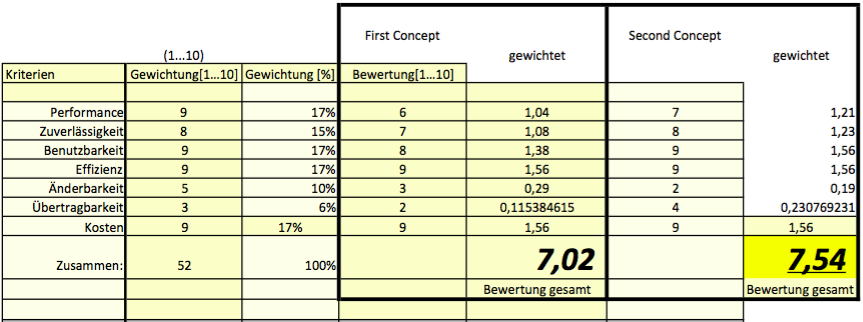
\includegraphics[scale=0.5]{images/Nutzwert.png}

\section {Conclusio}
Abschließend wird innerhalb der Festlegung der User Stories vor allem darauf zu achten sein möglichst wenige Eingaben vom User abzuverlangen und möglichst viel direkt aus der OBD2 Schnittstelle mittels der PID's zu bekommen, da dies ein großes Fehlerpotenzial bergen würde. 
Ein Framework wird auch sehr wichtig sein um die Arbeit an der App möglichst fehlerfrei und unterbrechungsfrei zu ermöglichen. Hierfür muss eine Testapplikation mit Ionic geschrieben werden um zu sehen ob es fehlerfrei genug ist um es während der Fahrt einsetzen zu können, da es hierfür möglichst wenige Fehler bergen sollte um den Fahrer nicht abzulenken. Andernfalls könnte man auf Firebase zurückgreifen.
